\section{Multiplatform Development}
One of the goals of this thesis project was to develop an app that supports both iOS and Android. This section describes implementation details specific to the respective operating systems.
\subsection{Tools used \& supported Versions}
\paragraph{Android}
The Android App is written in Java using Android Studio as the development environment.\\
The minimum required Version of Android is API Level 16. This minimum Version Number determines which devices can run the App. As of July 6, 2017 this will mean that 98,6\%~\cite{versions_Android} of all Android Users can download, install and run the App.
\paragraph{iOS}
The iOS Version was developed in Xcode using Swift. The UI was developed with a storyboard which "is a visual representation of the user interface of an iOS application, showing screens of content and the connections between those screens" \cite{story}.\\
Feedbacker on iOS supports all devices running iOS 9 or newer. This corresponds to 97\% of all App Store users \cite{versions_iOS}.

\subsection{Implementation of Firebase}\label{ssec:implementation}

\subsubsection{Initialization}
For both platforms Firebase has to be imported as an additional library. Furthermore the \textit{google-services} file needs to reside in the app's directory. This file can be downloaded after registering the app in the firebase console.\\

\paragraph{Android}
Importing Firebase on Android is achieved by adding the relevant Firebase dependencies to the gradle build file. Also the Google Play Services plugin needs to be applied.
\begin{listing}[H]
  \caption{Gradle Dependencies}
  \label{mint:grdl_dep}
  \begin{minted}[frame=lines, framesep=10pt, breaklines=true, breakbefore=.]{groovy}
dependencies{
  compile 'com.google.firebase:firebase-core:10.2.1'
  compile 'com.google.firebase:firebase-database:10.2.1'
  compile 'com.google.firebase:firebase-auth:10.2.1'
  ...
}
apply plugin: 'com.google.gms.google-services'
  \end{minted}
\end{listing}

\paragraph{iOS}
iOS manages third party SDKs and dependencies with so called pods. They are configured inside a podfile and installed using \mintinline{bash}{pod install} in the command line. This will create a \textit{.xcworkspace} file which has to be used for further development.\\
After that was done successfully Firebase needs to be initialized inside the App Delegate with \mintinline{swift}{FirebaseApp.configure()}.

\subsubsection{Usage}\label{ssec:usage}
As explained in section \ref{ssec:data_structure}, Firebase saves data in a JSON tree. Each node in this tree can be addressed as a \textit{DatabaseReference}. The following examples show how read and write operations work in Firebase. As the APIs for Android and iOS are similar only the iOS version is shown here.

\paragraph{Read Data}
Firebase reads data by attaching an observer to a \textit{DatabaseReference}. The example below shows how this was used to mark the user's feedback on the Map (Figure \ref{fig_map}).\\

\begin{listing}[H]
  \caption{Read Data}
  \label{mint:read_data}
  \begin{minted}[frame=lines, framesep=10pt, breaklines=true, breakafter=)]{swift}
func createPersonalMarkers(){
  let uid : String = (Auth.auth().currentUser?.uid)!
  let personalFeedbackRef : DatabaseReference = FirebaseHelper.ref.child("users").child(uid).child("feedback")
  //Observe personal Feedback Ref for new Childs
  personalFeedbackRef.observe(.childAdded, with: { snapshot in
    let id : String = snapshot.key
    FirebaseHelper.ref.child("feedback").child(id).observeSingleEvent(of: .value, with: { (snapshot) in
      //Create Feedback from snapshot and create Annotation
    })
  })
  //Observe personal Feedback Ref for changes
  personalFeedbackRef.observe(.childChanged, with: { snapshot in
    let id : String = snapshot.key
    FirebaseHelper.ref.child("feedback").child(id).observeSingleEvent(of: .value, with: { (snapshot) in
      //Create Feedback from snapshot and create Annotation
    })
  })
  //Observe personal Feedback Ref for new deleted Childs
  personalFeedbackRef.observe(.childRemoved, with: {snapshot in
    let id : String = snapshot.key
    // Code for deleting the marker
  })
}
  \end{minted}
\end{listing}

The way the data is structured for Feedbacker (see section \ref{ssec:data_structure}) the user only saves a reference to a feedback in his section of database. This means that when an object was added or changed the corresponding feedback needs to be read as well. This is also achieved by observing a \textit{DatabaseReference} for the selected feedback. It is a one-time-only meaning it only reads the data once and then it is detaching itself from the reference.\\
When a user toggles to not show his personal feedback (or published feedbacks) on the map the observer on the reference is detached. This system of permanent observers and one time only observers means that the network traffic for the user is kept at a minimum.


\paragraph{Write/Delete Data}
For both apps a FirebaseHelper class was written to save, delete feedback and create new IDs for Feedback. The following explains how this was achieved.

\begin{listing}[H]
  \caption{Save Feedback}
  \label{mint:save_feedback}
  \begin{minted}[frame=lines, framesep=10pt, breaklines=true, breakafter=)]{swift}
static func saveFeedback(feedback : Feedback){
  let uid : String = (Auth.auth().currentUser?.uid)!
  //Save Feedback in User Section
  ref.child("users").child(uid).child("feedback").child(feedback.id).setValue(feedback.category)
  //If made public save it in Published
  if(feedback.published){
    ref.child("published").child(feedback.id).setValue(feedback.category)
  } else{
    ref.child("published").child(feedback.id).removeValue()
  }
  //Save the Feedback itself
  ref.child("feedback").child(feedback.id).setValue(feedback.getDataAsDict())
}
  \end{minted}
\end{listing}
It is important to note that the feedback is saved in the user directory, the feedback directory, and, if it is published, in the published directory.

\begin{listing}[H]
  \caption{Delete Feedback}
  \label{mint:delete_feedback}
  \begin{minted}[frame=lines, framesep=10pt, breaklines=true, breakafter=)]{swift}
static func deleteFeedback(feedback : Feedback){
  let uid : String = (Auth.auth().currentUser?.uid)!
  ref.child("feedback").child(feedback.id).removeValue()
  ref.child("published").child(feedback.id).removeValue()
  ref.child("users").child(uid).child("feedback").child(feedback.id).removeValue()
}
  \end{minted}
\end{listing}
Similarly, references to the feedback need to be removed from all sections in the database when it is deleted.

\begin{listing}[H]
  \caption{Generate Feedback Id}
  \label{mint:create_feedback_id}
  \begin{minted}[frame=lines, framesep=10pt, breaklines=true, breakafter=)]{swift}
static func getFeedbackId() -> String {
  return ref.child("feedback").childByAutoId().key
}
  \end{minted}
\end{listing}
The Firebase \mintinline{swift}{childByAutoId()} is used to create IDs for feedbacks. According to the Firebase documentation, this command "generates a new child location using a unique key" \cite{autoID}. This means that every new feedback really has a unique ID and cannot be overridden by another user's feedback.

\subsection{Location}
\subsubsection{Location Permission}
In order to get access to the user's location data, both platforms demand apps to ask for permission by the user to do so.

\paragraph{Android}
Up until Android 6.0 (API 23) Permissions were granted on installation. This led to many users not installing certain apps due to uncertainty why apps would need access to services like location.\\

\begin{listing}[H]
  \caption{Android Manifest Location Permission}
  \label{mint:manifest_and}
  \begin{minted}[frame=lines, framesep=10pt, breaklines=true, breakbefore=.]{xml}
  <uses-permission android:name="android.permission.ACCESS_COARSE_LOCATION"/>
  <uses-permission android:name="android.permission.ACCESS_FINE_LOCATION"/>
  \end{minted}
\end{listing}
If an app wants to use certain features it has to define them in the app's manifest. As Feedbacker is targeting API Level 25 it needs to request permissions also at runtime. If the user already granted the permission nothing happens. If the user has yet to allow location access for the app a dialog is shown, prompting the user to grant location access.\\

\begin{listing}[H]
  \caption{Location Permission Android}
  \label{mint:loc_perm_and}
  \begin{minted}[frame=lines, framesep=10pt, breaklines=true, breakbefore=.]{java}
public void onRequestPermissionsResult(int requestCode, String[] permissions, int[] grantResults) {
  super.onRequestPermissionsResult(requestCode, permissions, grantResults);
  switch (requestCode) {
    case PERMISSION_LOCATION_REQUEST_CODE: {
      if (grantResults.length > 0 &&
        grantResults[0] == PackageManager.PERMISSION_GRANTED) {
        //Check if App has Hardware Permissions [True because of App Manifest]
          //then start Listening for Location Update
      } else {
        //Permission for Location was Denied
        // --> Switch To Error Fragment
      }
    }
  }
}
  \end{minted}
\end{listing}


\paragraph{iOS}
On iOS the Location Manager is in charge of handling location permissions.
\begin{listing}[H]
  \caption{Location Permission iOS}
  \label{mint:loc_perm_ios}
  \begin{minted}[frame=lines, framesep=10pt, breaklines=true, breakbefore=.]{swift}
let locationManager = CLLocationManager()
locationManager.requestAlwaysAuthorization()
locationManager.requestWhenInUseAuthorization()
  \end{minted}
\end{listing}
The Location Manager is requesting access to the location of the user. If the user has not granted permission yet or has revoked location access a dialog will prompt the user to give the app access to the location.
Furthermore the usage of location and the reasons for it have to be declared in the \textit{Info.plist} file.

\begin{figure}[H]
\begin{center}
  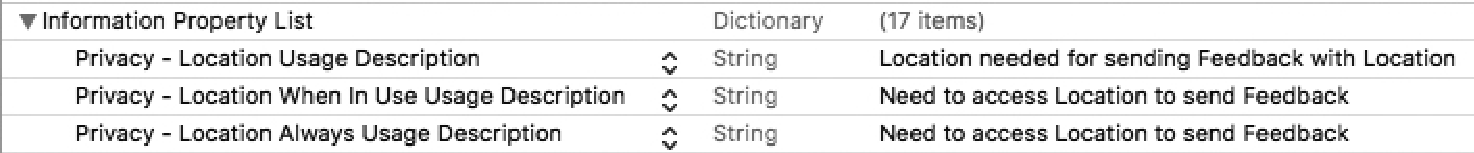
\includegraphics[width=400pt]{bilder/info_plist_location_bw.pdf}
  \caption{Location Permission flags in Info.plist}\label{infoplist_loc_perm}
\end{center}
\end{figure}


\subsubsection{Listening for Location Updates}
\paragraph{Android}
%%TODO: Link to GoogleApiClient and FusedLocationAPI Docs
Android's location updates are handled by a GoogleApiClient \cite{gAC} and the FusedLocationProviderAPI \cite{fla}.

\begin{listing}[H]
  \caption{Init Location Updates Android}
  \label{mint:loc_upd_and}
    \begin{minted}[frame=lines, framesep=10pt, breaklines=true, breakbefore=.]{java}
mLocationRequest = new LocationRequest();
//get new Location every 5-10 Seconds
mLocationRequest.setInterval(10000);
mLocationRequest.setFastestInterval(5000);
//Use highest Accuracy Possible
mLocationRequest.setPriority(LocationRequest.PRIORITY_HIGH_ACCURACY);
LocationSettingsRequest.Builder builder = new LocationSettingsRequest.Builder()
      .addLocationRequest(mLocationRequest).setAlwaysShow(true);
builder.build();
LocationServices.FusedLocationApi.requestLocationUpdates(mGoogleApiClient, mLocationRequest, this);
    \end{minted}
\end{listing}

First a location request is generated and configured (in this case with an update interval of 5-10 seconds, highest accuracy possible).

\begin{listing}[H]
  \caption{Location Changed Android}
  \label{mint:loc_changed_and}
    \begin{minted}[frame=lines, framesep=10pt, breaklines=true, breakbefore=.]{java}
@Override
public void onLocationChanged(Location location) {
  mCurrentLocation = location;
  mLastUpdateTime = Calendar.getInstance();
}
    \end{minted}
\end{listing}

This function is overridden from \mintinline{java}{com.google.android.gms.location.LocationListener} and is called every time the location changed.\\
If the location changed, the new location and the current time of the user's device will be saved.This information is accessed when a new feedback is created.

\paragraph{iOS}
Similar to Android first the location manager from Listing \ref{mint:loc_perm_ios} gets configured as desired.
\begin{listing}[H]
  \caption{Init Location Manager iOS}
  \label{mint:loc_mgr_ios}
    \begin{minted}[frame=lines, framesep=10pt, breaklines=true, breakbefore=.]{swift}
locationManager.delegate = self
locationManager.desiredAccuracy = kCLLocationAccuracyNearestTenMeters
locationManager.startUpdatingLocation()
    \end{minted}
\end{listing}

Also similar to Android a function is overridden to handle the callback when the location changed.
\begin{listing}[H]
  \caption{Location Changed iOS}
  \label{mint:loc_changed_ios}
    \begin{minted}[frame=lines, framesep=10pt, breaklines=true, breakbefore=.]{swift}
func locationManager(_ manager: CLLocationManager, didUpdateLocations locations: [CLLocation]) {
  let location = locations[0]
  coordinate = location.coordinate
  date = location.timestamp
}
    \end{minted}
\end{listing}
This function is implemented from \mintinline{swift}{CLLocationManagerDelegate}. Like in Listing \ref{mint:loc_changed_and} the new location and time are saved and accessed when creating a new feedback.

\subsection{Internationalization}
In order to give users the best experience possible it is best practice in App development to offer the App in as many Languages as possible. Both platforms Android and iOS achieve this by storing the strings to be displayed in the user interface in special language files.\\
The system then automatically chooses which string to pick and display to the user.\\
At the moment of releasing this thesis, Feedbacker supports English and German.

\paragraph{Android}
On Android the strings are saved in \textit{values/strings.xml} for the
standard translation (english) and in \textit{values-de/strings.xml} for german. Additional translations would be saved in a folder with the respective country code. This system also allows having different resource values like margins in layout for different regions.\\
\begin{listing}[H]
  \caption{Strings Android English}
  \label{mint:strings_and_eng}
    \begin{minted}[frame=lines, framesep=10pt, breaklines=true, breakbefore=.]{xml}
<string name="cat_neg_dark">Dark Place</string>
<string name="cat_neg_dirty">Dirty</string>
    \end{minted}
\end{listing}
The strings are identified by a key that is common to all languages implemented.
\begin{listing}[H]
  \caption{Strings Android German}
  \label{mint:strings_and_ger}
    \begin{minted}[frame=lines, framesep=10pt, breaklines=true, breakbefore=.]{xml}
<string name="cat_neg_dark">Dunkler Ort</string>
<string name="cat_neg_dirty">Dreckig</string>
    \end{minted}
\end{listing}
That is, the German strings all have the same key as the English counterparts with only the value changing according to the translation.\\


\paragraph{iOS}
iOS also utilizes special files to support different languages. The languages wanted have to be declared in the info section of the project settings.\\
This will then create \textit{*.string} files for the storyboard selected.\\
\begin{listing}[H]
  \caption{Strings iOS English}
  \label{mint:strings_ios_eng}
    \begin{minted}[frame=lines, framesep=10pt, breaklines=true, breakbefore=.]{java}
/* Class = "UITabBarItem"; title = "Map"; ObjectID = "cPa-gy-q4n"; */
"cPa-gy-q4n.title" = "Map";
/* Class = "UITabBarItem"; title = "Profile"; ObjectID = "kUv-uF-GHa"; */
"kUv-uF-GHa.title" = "Profile";
    \end{minted}
\end{listing}

Similar to Android all UI-Strings have a common key and the value according to the language.
\begin{listing}[H]
  \caption{Strings iOS German}
  \label{mint:strings_ios_ger}
    \begin{minted}[frame=lines, framesep=10pt, breaklines=true, breakbefore=.]{java}
/* Class = "UITabBarItem"; title = "Map"; ObjectID = "cPa-gy-q4n"; */
"cPa-gy-q4n.title" = "Karte";
/* Class = "UITabBarItem"; title = "Profile"; ObjectID = "kUv-uF-GHa"; */
"kUv-uF-GHa.title" = "Profil";
    \end{minted}
\end{listing}

The app will automatically display the UI with the language selected by the user in the system settings.\\
Localized strings required outside of the UI are saved in \textit{localized.string} similar to the storyboard and UI relevant files they get sub level files for each language. These Strings can be accessed project-wide with \mintinline{swift}{NSLocalizedString("cat_neg_dark", comment: NEG_DARK)}.
